\capitulo{5}{Aspectos relevantes del desarrollo del proyecto}

En este apartado se van a recoger los aspectos más importantes del
desarrollo del proyecto. Desde las decisiones que se tomaron y sus
implicaciones, hasta los numerosos problemas a los que hubo que
enfrentarse y cómo se solucionaron.

\section{Inicio del proyecto}\label{inicio-del-proyecto}

La idea del proyecto surgió del afán de encontrar un tema con el que
poder aunar mi formación técnica y mis aficiones.

Mi padre me transmitió el interés por la apicultura desde bien pequeño
y, posteriormente, llegué a trabajar en una empresa de apicultura
profesional. Esto me hizo ser consciente de los problemas con los que
lidia día a día un apicultor. Por otro lado, los conocimientos
adquiridos durante mis estudios de Ingeniería Informática, me
posibilitaron idear soluciones tecnológicas a alguno de estos problemas.

Tras formalizar la idea del proyecto y recibir el visto bueno de los
tutores, nos pusimos manos a la obra.

\begin{figure}[H]
	\centering
	
\includegraphics[width=0.4\textwidth]{GoBees_logo}
	\caption{Logo de GoBees.}
	\label{fig:logo}
\end{figure}

\section{Metodologías}\label{metodologias-proyecto}

Desde el primer momento se dedicaron grandes esfuerzos para que la
realización del proyecto se llevase a cabo de la manera más profesional
posible. Para ello, se siguieron varias metodologías y procesos,
expuestos a continuación.

Para la gestión del proyecto se utilizó una metodología ágil, en
concreto Scrum. Aunque no se siguió al 100\% al tratarse de un proyecto
educativo (no éramos un equipo de 4 a 8 personas, no hubo reuniones
diarias, etc.), sí que se aplicó una filosofía ágil en líneas generales:

\begin{itemize}
\tightlist
\item
  Se siguió una estrategia de desarrollo incremental a través de
  iteraciones (\emph{sprints}) y revisiones.
\item
  La duración media de los \emph{sprints} fue de una semana.
\item
  Al finalizar cada \emph{sprint} se entregaba una parte del producto
  operativo (incremento).
\item
  Se realizaban reuniones de revisión al finalizar cada \emph{sprint} y
  al mismo tiempo de planificación del nuevo \emph{sprint}.
\item
  En la planificación del \emph{sprint} se generaba una pila de tareas a
  realizar.
\item
  Estas tareas se estimaban y priorizaban en un tablero \emph{canvas}
  (ZenHub).
\item
  Para monitorizar el progreso del proyecto se utilizó gráficos
  \emph{burndown}.
\end{itemize}

Para el diseño del algoritmo de visión artificial se utilizó una
metodología de ensayo y error. Se barajaban diferentes alternativas y se
iban verificando empíricamente su eficacia y eficiencia.

Para el desarrollo de la aplicación Android se intentó utilizar
\emph{Test-Driven Development} (TDD) para fomentar la escritura de test
y mejorar la calidad del \emph{software}. La mayoría de los módulos de
la aplicación se implementaron exitosamente siguiendo esta metodología.
Sin embargo, en las partes más complejas de esta, como el servicio de
monitorización, se hacía muy engorroso la escritura de test (ya
complicada de por sí en Android), por lo que finalmente se omitieron al
penalizar notablemente la productividad.

\section{Formación}\label{formacion}

El proyecto requería una serie de conocimientos técnicos de los que no
se disponía en un principio. Sobre todo, relacionados con visión
artificial, OpenCV y Android. A continuación, se enumeran los
principales recursos didácticos que se utilizaron.

Para la formación en visión artificial y OpenCV se leyeron los
siguientes libros:

\begin{itemize}
\tightlist
\item
  \emph{Android Application Programming with OpenCV 3} (Joseph Howse)
  \citep{book:android_opencv}.
\item
  \emph{Mastering OpenCV Android Application Programming} (Salil Kapur y
  Nisarg Thakkar) \citep{book:mastering_opencv}.
\item
  \emph{Learning Image Processing with OpenCV} (Ismael Serrano Gracia,
  Jesús Salido Tercero y José Luis Espinosa Aranda)
  \citep{book:learning_cv}.
\item
  \emph{OpenCV 3.0 Computer Vision with Java} (Daniel Lélis Baggio)
  \citep{book:opencv_java}.
\end{itemize}

Para la formación en Android se realizaron los siguientes cursos online:

\begin{itemize}
\tightlist
\item
  \emph{Android Development for Beginners: How to Make Apps} (Udacity)
  \citep{course:android_beginners}.
\item
  \emph{Developing Android Apps} (Udacity)
  \citep{course:developing_android}.
\item
  \emph{Android Testing Codelab} (Google) \citep{course:testing}.
\end{itemize}

También cabe destacar la importancia que tuvo la comunidad
\href{http://stackoverflow.com/}{StackOverflow} para la resolución de
los diferentes problemas que surgieron durante el desarrollo.

\section{Desarrollo del algoritmo}\label{desarrollo-del-algoritmo}

Una gran parte de los recursos del proyecto se dedicaron al desarrollo
del algoritmo de visión artificial para la monitorización de la
actividad de vuelo de una colmena.

El problema a resolver poseía una serie de condicionantes que
dificultaban el análisis:

\begin{itemize}
\tightlist
\item
  Cada abeja ocupa una porción muy pequeña de la imagen.
\item
  Las condiciones lumínicas varían a lo largo del día o de la época del
  año.
\item
  Existen sombras producidas por la cámara o por las propias abejas.
\item
  A 20 fps una abeja volando puede recorrer una distancia significativa
  entre fotogramas.
\item
  Un grupo de abejas puede estar confinado, dificultando su
  segmentación.
\end{itemize}

El desarrollo comenzó con una búsqueda bibliográfica sobre el tema. En
esta, se encontraron varios artículos relacionados que nos dieron una
idea de las técnicas que podíamos probar. También se tuvo una reunión
con un experto en visión artificial que nos proporcionó su punto de
vista sobre cómo abordar el problema.

El primer punto a abordar fue la toma de las imágenes. Se decidió que la
toma se debía de hacer con un trípode en posición cenital a la colmena.
De esta manera, se disminuía las diferencias de tamaño por perspectiva,
no se obstaculizaba el vuelo de las abejas y se facilitaba el análisis.
Además, era aconsejable cubrir el suelo con alguna superficie uniforme
para mejorar la segmentación de las abejas.

\imagen{cenital}{Colocación del \emph{smartphone} en la colmena.}

En un primer momento, el desarrollo del algoritmo se iba a realizar
directamente sobre la plataforma Android. Sin embargo, rápidamente nos
dimos cuenta que no era lo más adecuado si queríamos seguir una
metodología basada en el ensayo y error, debido a los elevados tiempos
de compilación y a la poca flexibilidad de la plataforma.

Finalmente se decidió desarrollar el algoritmo directamente en Java, ya
que nos proporcionaba una mayor flexibilidad y, además, migrar el código
a Android posteriormente sería una tarea bastante trivial.

Para facilitar el desarrollo del algoritmo y del testeo de las
diferentes alternativas se realizó una aplicación Java (ver \ref{fig:devplatform1}) 
que permitía parametrizar en tiempo real las diferentes etapas del algoritmo.
Además, se podía observar la salida de cada etapa del algoritmo y su tiempo de
computación.

Es importante recalcar que los tiempos de computación obtenidos en la
plataforma había que multiplicarlos por cuatro si se quería obtener una
estimación de lo que equivaldría ejecutarlo en el dispositivo móvil. Por
lo que los márgenes con los que se jugaba no eran demasiado grandes.

\begin{figure}[H]
	\centering
	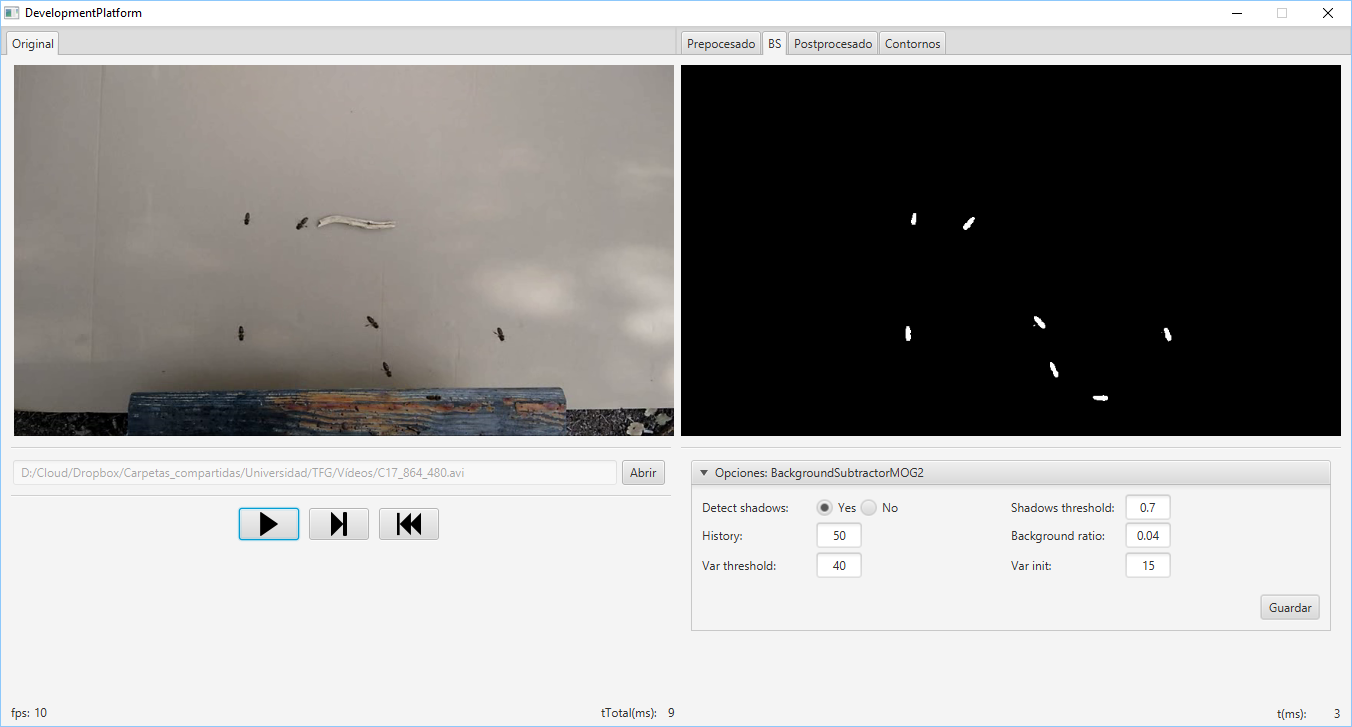
\includegraphics[width=0.9\textwidth]{devplatform}
	\caption{Plataforma de desarrollo del algoritmo.}
	\label{fig:devplatform1}
\end{figure}

Tras varias iteraciones, se consiguió obtener un algoritmo bastante
robusto que poseía las siguientes etapas:

\begin{enumerate}
\def\labelenumi{\arabic{enumi}.}
\tightlist
\item
  \textbf{Preprocesado:} conversión de RGB a escala de grises y
  desenfoque Gaussiano para facilitar el procesado.
\item
  \textbf{Substracción del fondo:} extracción de los elementos en
  movimiento utilizando el algoritmo \texttt{BackgroundSubtractorMOG2}.
\item
  \textbf{Posprocesado:} mejora de la salida de la etapa anterior
  mediante varias iteraciones de erosión y dilatación.
\item
  \textbf{Detección y conteo de abejas:} localización de los contornos
  pertenecientes a abejas en base al área y conteo de los mismos.
\end{enumerate}

\section{Desarrollo de la \emph{app}}\label{desarrollo-de-la-app}

El desarrollo de la aplicación Android se realizó de forma incremental,
publicando una \emph{release} al finalizar cada \emph{sprint}.

Se decidió dar soporte a partir de la versión KitKat (API 19), de tal
forma que se cubría un 86,3\% de los dispositivos Android del mercado
\citep{android:versions}. Dar soporte a versiones anteriores suponía una 
sobrecarga importante, por lo que se descartó al no constituir una cuota de
mercado importante.

La primera tarea consistió en migrar el algoritmo de visión artificial a
la plataforma Android. A primera vista, no parecía una tarea complicada.
Sin embargo, nos encontramos con varios \emph{bugs} que, unidos a la
mala documentación de OpenCV para Android, dificultó considerablemente
la labor.

El primer \emph{bug} (\emph{issue}
\href{https://github.com/davidmigloz/go-bees/issues/26}{\#26}) consistía
en que al llamar a algunas funciones del núcleo de OpenCV, se producía
un error con un mensaje que hacía referencia a una señal que variaba
entre ejecuciones, lo cual hizo muy difícil encontrar el origen.
Finalmente, se dio con la fuente del problema, el cual tenía su origen
en que la versión de la aplicación OpenCV Manager distribuida en el
Google Play contaba con una versión corrupta de la librería OpenCV 3.1.

Se notificó al equipo de OpenCV a través de su gestor de incidencias y
finalmente solucionaron el problema en la nueva versión OpenCV 3.2.

El segundo \emph{bug} (\emph{issue}
\href{https://github.com/davidmigloz/go-bees/issues/27}{\#27}) hacía que
la aplicación fallase cuando se compilaba para dispositivos con una
versión de Android inferior a Lollipop, debido a la API de la cámara.
Tras publicar el caso en
\href{http://stackoverflow.com/questions/39770355/classnotfoundexception-android-hardware-camera2-cameraaccessexception-with-open}{StackOverflow},
un usuario sugirió que podía estar relacionado con el \emph{Instant Run}
de Android Studio. Y así fue; desactivando esta característica, la
aplicación no fallaba. Se describió el caso en el gestor de incidencias
de Android y, a día de hoy (enero 2017), el \emph{bug} se encuentra
resuelto y está a la espera de ser incorporado en futuras
\emph{releases} del \emph{framework}.

Una vez solventados ambos \emph{bugs,} se logró que el algoritmo
funcionase sin problemas en la nueva plataforma.

Cabe destacar que como OpenCV no distribuía oficialmente la librería a
través de ningún repositorio que permitiese utilizarla directamente como
dependencia Gradle, se creó uno propio \citep{gobees:prototipes}.

Para el diseño de la arquitectura de la \emph{app} se siguió el patrón
de arquitectura \emph{Model-View-Presenter} (MVP), que permite separar
los datos internos del modelo de una vista pasiva y agrupar toda la
lógica de la aplicación en una capa intermedia llamada \emph{presenter}.
De esta manera se consigue un código muy desacoplado, haciendo que este
sea más fácil de testear y mantener.

En cuanto a la persistencia de datos, se optó por utilizar Realm. Se
trata de una base de datos orientada a objetos que proporciona una API
para trabajar directamente con la capa de persistencia. Es
multiplataforma y presume de ser más rápida que SQLite.

Para la obtención de la información meteorológica se escogió la API
proporcionada por \emph{OpenWeatherMaps}, la cual nos permitía realizar
hasta 60 llamadas por minuto de forma gratuita.

El acceso a datos se centralizó utilizando el patrón repositorio, que
abstrae la lógica de negocio de la fuente de datos. Todo el acceso a
datos se centraliza en el repositorio y es este quien decide de qué
fuente los obtiene (base de datos, internet, etc.). Además, se incorporó
una capa de caché en este punto con el fin de agilizar la navegación por
la \emph{app}.

El siguiente esquema resume la arquitectura de la aplicación:

\imagen{architecture}{Arquitectura de la aplicación.}

Surgieron problemas al implementar el algoritmo de monitorización como
un servicio de Android para que el usuario pudiese apagar la pantalla
durante la monitorización. El acceso a la cámara proporcionado por
OpenCV era en sí una vista, y las vistas no pueden ser utilizadas en
servicios. Finalmente se optó por realizar una implementación propia que
accediese directamente a la API de la cámara y convirtiese los
fotogramas al formato de OpenCV.

En cuanto al diseño de la aplicación, se dedicaron grandes esfuerzos a
la usabilidad y accesibilidad de la misma. Se siguieron las directrices
de diseño recogidas en la guía de Material Design en cuanto a estilos,
disposición de los elementos, tipos de componentes, patrones de
navegación, gestos, etc.

Por último, se internacionalizó la aplicación a los siguientes idiomas:
español, inglés, catalán, polaco y árabe. Para ello se utilizó la
herramienta Toolkit del Traductor de Google que permite realizar una
primera traducción automática de los diferentes textos de la aplicación
y posteriormente una revisión colaborativa de los resultados de esta.
Para la revisión se recurrió a amistades nativas en los diferentes
idiomas.

\section{\emph{Testing}}\label{testing}

En lo relativo al \emph{testing}, podemos diferenciar el testeo del
algoritmo del testeo de la \emph{app}.

Para testear el error cometido por el algoritmo era necesario contar con
fragmentos de vídeo etiquetados con el número de abejas presentes en
cada fotograma. Como esta labor era muy tediosa, se desarrolló una
aplicación Java (ver \ref{fig:counting_platform}) para agilizar 
el etiquetado de los fotogramas.

La aplicación iba mostrando los diferentes fotogramas al usuario y este
indicaba con el ratón los píxeles pertenecientes a abejas. Finalmente
permitía exportar los datos en un archivo CSV.

\begin{figure}[H]
	\centering
	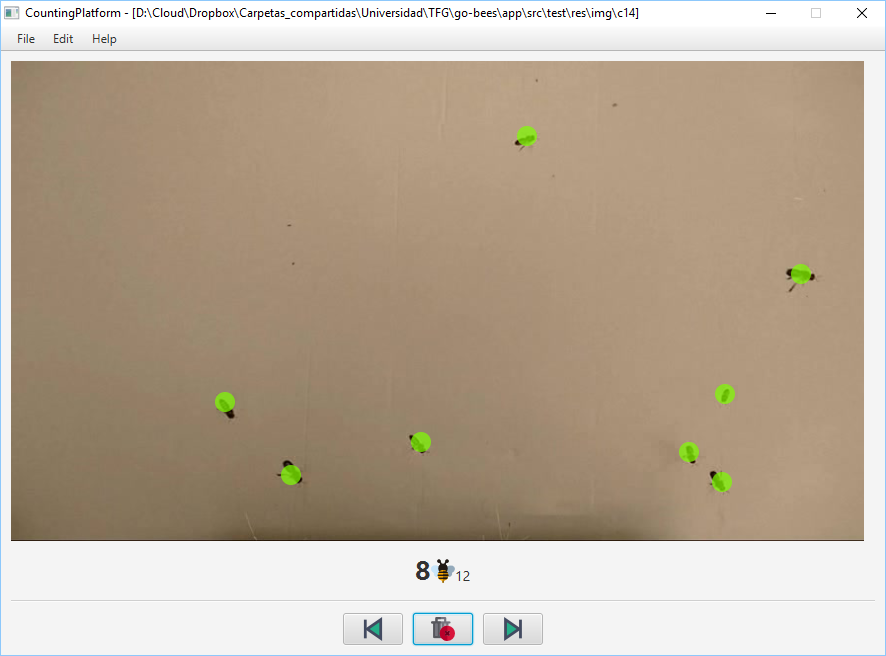
\includegraphics[width=\textwidth]{counting_platform}
	\caption{Plataforma de conteo de abejas}\label{fig:counting_platform}
\end{figure}

Se etiquetaron fragmentos de vídeo correspondientes a tres situaciones
distintas:
\newpage
\begin{itemize}
\tightlist
\item
  \textbf{Caso 1} (vídeo \href{https://youtu.be/9pkPCnS2aRY}{\#C14}):
  actividad media, sombras de abejas y moscas.
\item
  \textbf{Caso 2} (vídeo \href{https://youtu.be/ENocXS3cEP0}{\#C17}):
  actividad media, cambios de iluminación y sombras de árboles.
\item
  \textbf{Caso 3} (vídeo \href{https://youtu.be/YjGX4mC7pO4}{\#C5}):
  alta actividad, solapamiento, sombras y fondo no uniforme.
\end{itemize}

Tras ejecutar el algoritmo se obtuvieron los siguientes errores
relativos (considerando como error absoluto la distancia entre la medida
esperada y la obtenida):

\begin{itemize}
\tightlist
\item
  \textbf{Caso 1:} 2,43\%.
\item
  \textbf{Caso 2}: 0,89\%.
\item
  \textbf{Caso 3}: 4,48\%.
\end{itemize}

Se puede observar que en la situación menos favorable el error es menor
a un 5\%, precisión más que suficiente para la finalidad de los datos.

En cuanto al tiempo medio de ejecución del algoritmo para cada fotograma
era de 25 ms en el equipo de pruebas (Intel i7-3610QM) y de 100 ms
cuando se ejecutaba en un \emph{smartphone} (Xiaomi Mi4).

Por otra parte, la aplicación se testeó mediante test unitarios, test de
integración y test de interfaz. La mayor parte de los test unitatios se
realizaron contra los \emph{presenters}, que son los que poseen la
lógica de negocio de la \emph{app}. Se realizó un test de interfáz por 
cada requisito y se se ejecutaron en siete dispositivos diferentes, uno por 
cada versión de Android que soporta la \emph{app} (API 19-25).

Además, se configuraron una serie de servicios de integración continua,
de tal forma, que cada vez que se realizaba un \emph{commit} en el
repositorio, se ejecutaban las siguientes tareas:

\begin{enumerate}
\def\labelenumi{\arabic{enumi}.}
\tightlist
\item
  \textbf{Travis}: realizaba una compilación del proyecto, ejecutaba los
  test unitarios, ejecutaba \emph{Lint}, ponía en marcha un emulador de
  Android, y ejecutaba los Android test sobre este. Al finalizar,
  enviaba los resultados a Codecov y SonarQube.
\item
  \textbf{Codecov}: realizaba un análisis sobre la cobertura de los test
  unitarios.
\item
  \textbf{CodeClimate}: ejecutaba cuatro motores de chequeo
  (\emph{checkstyle}, \emph{fixme}, \emph{pmd} y \emph{markdownlint})
  sobre el código para detectar posibles problemas o vulnerabilidades en
  él.
\item
  \textbf{SonarQube}: analizaba código duplicado, violaciones de
  estándares, cobertura de tests unitarios, \emph{bugs} potenciales, etc.
\item
  \textbf{VersionEye}: chequeaba todas las dependencias utilizadas en la
  aplicación y comprobaba si estaban actualizadas, si tenían algún
  problema de seguridad conocido, o si violaban la licencia del
  proyecto.
\end{enumerate}

\begin{figure}[!h]
	\centering
	
\includegraphics[width=\textwidth]{ci}
	\caption{Servicios de integración continua.}\label{fig:ci}
\end{figure}

Por último, cabe comentar algunas estadísticas del proyecto:

\begin{table}[H]
\centering
\begin{tabular}{lr}
\toprule
\textbf{Concepto}                  & \multicolumn{1}{r}{\textbf{Valor}} \\ 
\midrule
Ratio de fiabilidad                & A          												\\
Ratio de seguridad                 & A																	\\
Ratio de mantenibilidad						 & A																  \\ 
\midrule
Número de clases Java              & 157                                \\
Número de archivos XML             & 96                                 \\
\midrule
Total de líneas Java               & 20.732                             \\
Líneas de código                   & 58\%            				            \\
Comentarios                        & 29\%          			                \\
Líneas en blanco                   & 13\%    		                        \\
\midrule
Número de test unitarios           & 120																\\
Cobertura total test unitarios     & 35,8\%                             \\
Cobertura test unitarios algoritmo & 100\%                              \\
Número de UI test                  & 17																	\\ 
\bottomrule
\end{tabular}
\caption{Estadísticas del proyecto.}
\label{stats}
\end{table}

\emph{*Los datos han sido obtenidos de los informes proporcionados por SonarQube y AndroidStudio.}

\section{Documentación}\label{aspectos-documentacion}

En un primer momento, se decidió escribir la documentación en formato
Markdown, utilizando las \emph{wikis} que proporciona GitHub en el
repositorio. De esta forma, la documentación podía ser visualizada
directamente desde GitHub, sin necesidad de tener que compilarla con
cada modificación.

Posteriormente, se optó por implementar un sistema de documentación
continua integrado en el repositorio, en concreto ReadTheDocs. De tal
forma, que la documentación se escribía en archivos Markdown dentro del
repositorio y este servicio generaba una página web
(\href{http://go-bees.readthedocs.io/}{go-bees.readthedocs.io}) que se
actualizaba cada vez que se realizaba un \emph{commit}.

No obstante, los tutores preferían obtener la documentación en formato
PDF para su corrección, por lo que finalmente se optó por utilizar
Sphinx junto con ReadTheDocs.

Sphinx es un generador de documentación que permite exportar la
documentación en varios formatos, entre ellos HTML y PDF.
Desafortunadamente, no soporta Markdown como formato de entrada, por
lo que hubo que migrar la documentación al formato reStructuredText.
Esta conversión se realizó con la herramienta Pandoc.

Con todo configurado, ahora ReadTheDocs generaba automáticamente la
página web (\ref{fig:readthedocs}) y un PDF actualizado con los 
últimos cambios realizados en la documentación.

\imagen{readthedocs}{Página web de documentación generada con ReadTheDocs.}

Para la exportación final de la memoria se utilizó el conversor Pandoc,
con objeto de transformar la documentación del formato reStructuredText
a \LaTeX. Algunos elementos, como las citas o las imágenes, no eran
convertidos correctamente, por lo que se tuvo que hacer uso de
expresiones regulares.

La totalidad de este tedioso proceso se realizó bajo la idea de que
cualquier proyecto comercial tiene su documentación accesible desde una
página web, y que además necesita estar acorde con la versión del
proyecto. Sin embargo, para este caso concreto en el que el entregable
final es un PDF con un formato determinado, el montar todo este sistema
ha supuesto una sobrecarga notable.

\section{Publicación}\label{publicacion}

En cuanto la aplicación estuvo lista para pasar a producción, se publicó
en la plataforma de distribución de aplicaciones Google Play.

\begin{figure}[H]
		\centering
	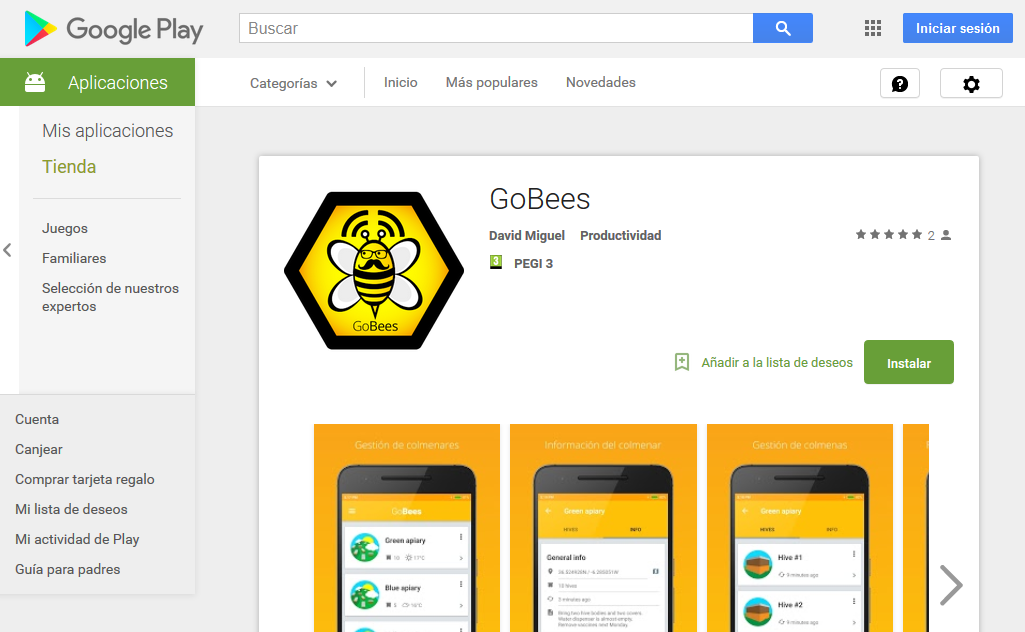
\includegraphics[width=\textwidth]{gobees-google-play}
	\caption{GoBees en Google Play.}\label{fig:gobees-google-play}
\end{figure}

Además, se desarrolló una página web promocional
(\href{http://gobees.io/}{gobees.io}), donde se describen las
características de la aplicación, los manuales de usuario, y el enlace
de descarga, entre otras cosas.

Por último, se crearon perfiles en las principales redes sociales para
promocionar la aplicación.

\section{Reconocimientos}\label{reconocimientos}

Durante el desarrollo del proyecto se obtuvieron varios reconocimientos:

\begin{itemize}
\tightlist
\item
  \textbf{Beca de colaboración con departamentos}: se me concedió esta
  beca para profundizar en el algoritmo desarrollado y publicar un
  artículo científico sobre él.
\item
  \textbf{Prototipos Orientados al Mercado}: GoBees resultó ganador de
  uno de los tres premios de la convocatoria de Prototipos Orientados al
  Mercado realizada por el Vicerrectorado de Investigación y
  Transferencia del Conocimiento~de la Universidad de Burgos.
\item
  \textbf{YUZZ}: GoBees fue elegido para participar en el programa YUZZ
  2017, patrocinado por el Banco Santander para el impulso del talento
  joven y el espíritu emprendedor.
\end{itemize}
